% Copyright (c) 2015 Benito Palacios Sánchez - All Rights Reserved.
% Esta obra está licenciada bajo la Licencia Creative Commons Atribución 4.0
% Internacional. Para ver una copia de esta licencia, visita
% http://creativecommons.org/licenses/by/4.0/.

\appendix
\backupbegin

\section{\appendixname}

\frame{\tableofcontents}

\begin{frame}
    \begin{alertblock}{Andew Huang - Hacking the Xbox. An introduction to Reverse Engineering}
        In general, I hack because it is quite satisfying to know that somebody's life was made better by something I built. I feel it is my obligation to apply my talents and return to society what it has given me. I also enjoy the challenge of exploration. I want to understand electronics as deeply as I can. Black boxes frustate me; nothing gets my curiosity going more than a box that I'm not allowed to open or understand. As a result, I have a fiduciary interest in cryptography and security methods.
    \end{alertblock}
\end{frame}

\subsection{Metodología}
\begin{frame}{Averiguar codificación desde tipografía}

\end{frame}

\subsection{Traducciones no oficiales}
\begin{frame}{Pokémon Perla y Diamante}
    % TODO: Añadir formato de texto.
\end{frame}

\begin{frame}{Pokémon HeartGold y SoulSilver}

\end{frame}

\begin{frame}{Pokémon Conquest}

\end{frame}

\begin{frame}{Ninokuni: El Mago de las Tinieblas}

\end{frame}

\subsection{Contenidos con derechos de autor}
\begin{frame}{100 Classic Book Collection}

\end{frame}

\begin{frame}{Elite Beat Agents}

\end{frame}

\begin{frame}{Guitar Rock}

\end{frame}


\subsection{Servicios en línea}
\begin{frame}{HMAC}
    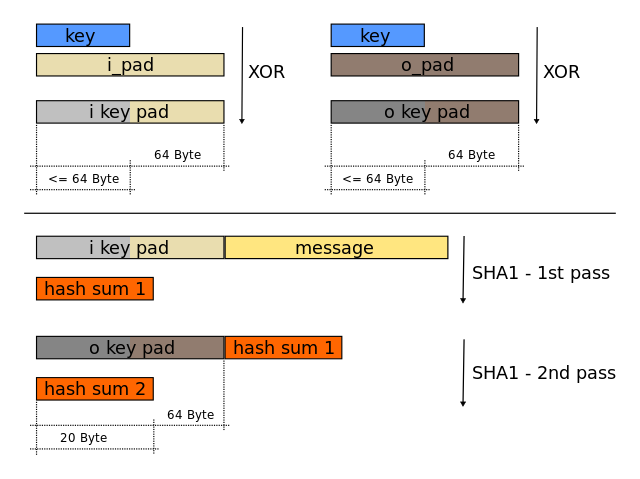
\includegraphics[width=\textwidth,height=0.8\textheight,keepaspectratio]{imgs/hmac.png}
\end{frame}

\begin{frame}{Servidores de Nintendo}
\textit{Token} generando aplicando \texttt{MD5} a:
\begin{columns}

\begin{column}{0.33\textwidth}\begin{itemize}
    \item \texttt{MD5} del \textit{challenge}$_{NAS}$.
    \item \textit{challenge}$_{consola}$.
\end{itemize}\end{column}

\begin{column}{0.33\textwidth}\begin{itemize}
    \item 48 espacios en blanco.
    \item \textit{challenge}$_{servidor}$.
\end{itemize}\end{column}

\begin{column}{0.33\textwidth}\begin{itemize}
    \item \textit{token}$_{NAS}$.
    \item \texttt{MD5} del \textit{challenge}$_{NAS}$.
\end{itemize}\end{column}

\end{columns}
\end{frame}

\begin{frame}{100 Classic Book Collection}

\end{frame}

\begin{frame}{Ninokuni: El Mago de las Tinieblas}

\end{frame}

\backupend
